\chapter{Grundlagen}

Dieses Kapitel soll technologische und konzeptionelle Grundlagen für die Studienarbeit liefern.
Zuerst werden anhand eines Beispiels Groupware-Systeme und deren Funktionalitäten dargestellt, um ein Verständnis für die Funktionsweise von Groupware-Systemen zu schaffen.
Daraufhin wird die Open-Source-Bibliothek Playwright vorgestellt, die in dieser Studienarbeit für die Implementierung von automatisierten End-to-End-Tests verwendet wurde.
Dabei wird auf die Gründe und Vorteile von End-to-End-Tests sowie die Funktionsweise von Playwright eingegangen.

\section{Groupware-Systeme}

Groupware-Systeme sind Software-Systeme, welche die Zusammenarbeit von Benutzern mit verschiedenen Tools zur gemeinsamen Kommunikation und Organisation unterstützen.
Dabei werden üblicherweise Funktionalitäten wie Kalender, Terminplanung, E-Mail und Kontaktmanagement bereitgestellt.

Im Folgenden werden anhand von Screenshots aus Microsoft Outlook-Live einige essenzielle Funktionen von Groupware-Systemen dargestellt und erklärt.
\begin{figure}[H]
    \centering
    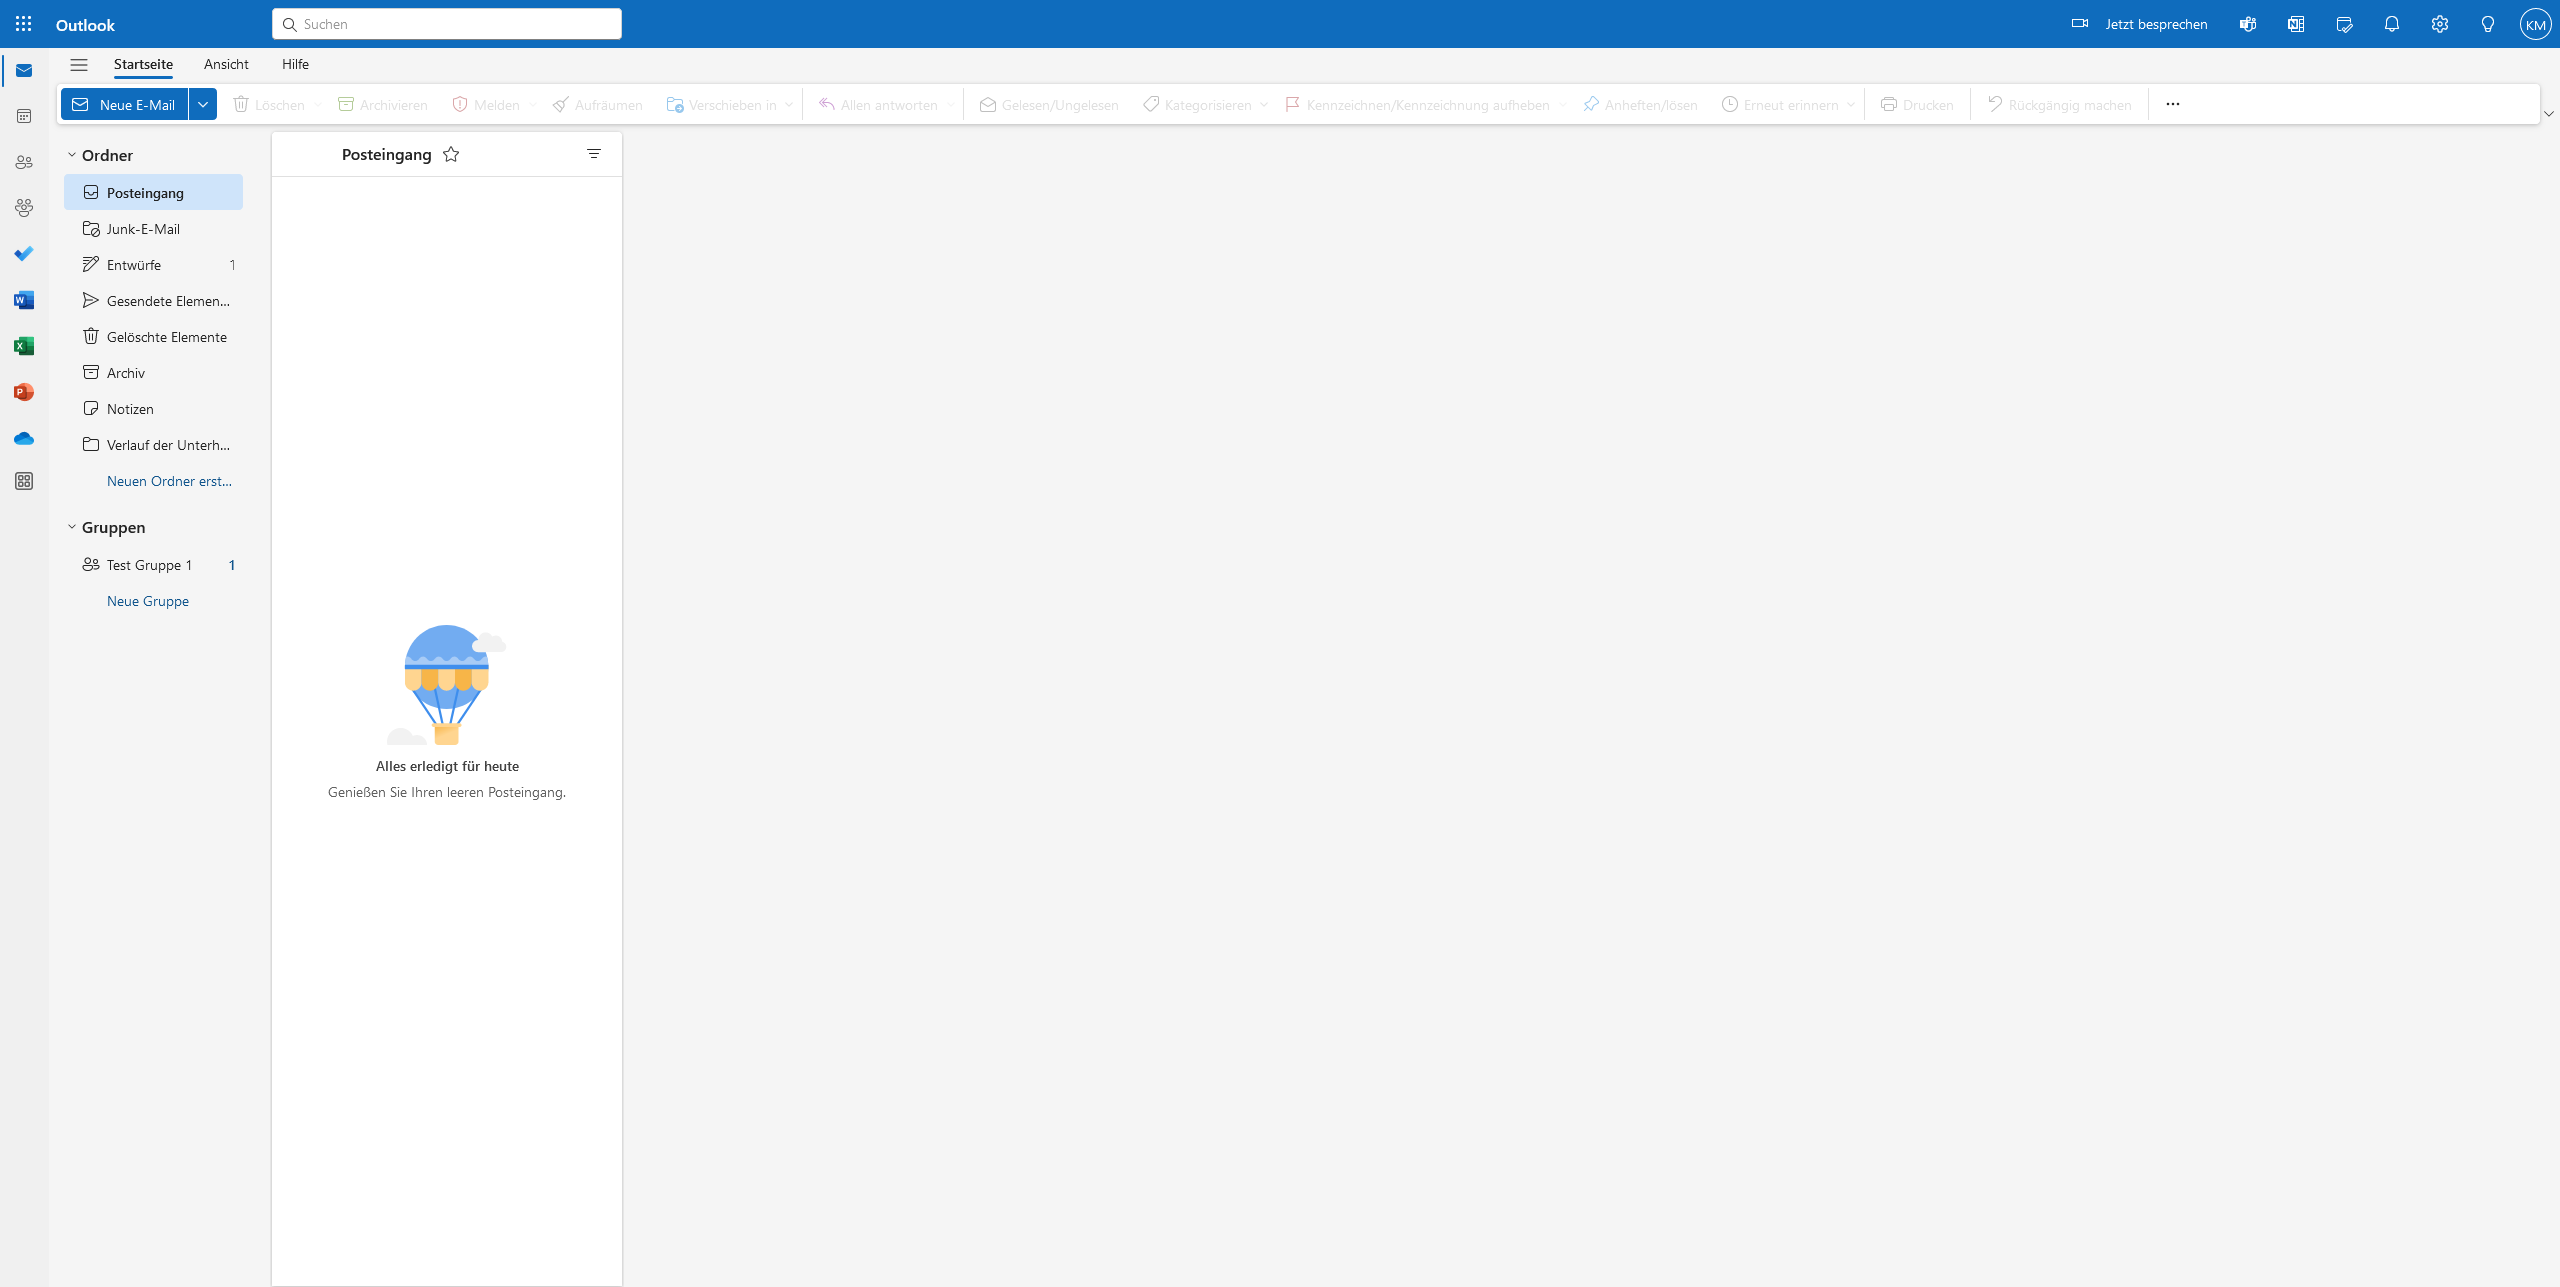
\includegraphics[width=0.75\textwidth]{images/OutlookLive_Mail1.png}
    \caption{Outlook-Live Mail}
    \label{fig:outlook-live-mail}
\end{figure}
Die erste Hauptfunktion von Groupware-Systemen besteht darin, einen E-Mail-Client bereitzustellen, über den E-Mails empfangen, versendet und verwaltet werden können. Dies wird beispielhaft anhand von Outlook-Live in Abbildung \ref{fig:outlook-live-mail} dargestellt.
Es sollte möglich sein, mehrere E-Mail-Postfächer gleichzeitig hinzuzufügen.


\begin{figure}[H]
    \centering
    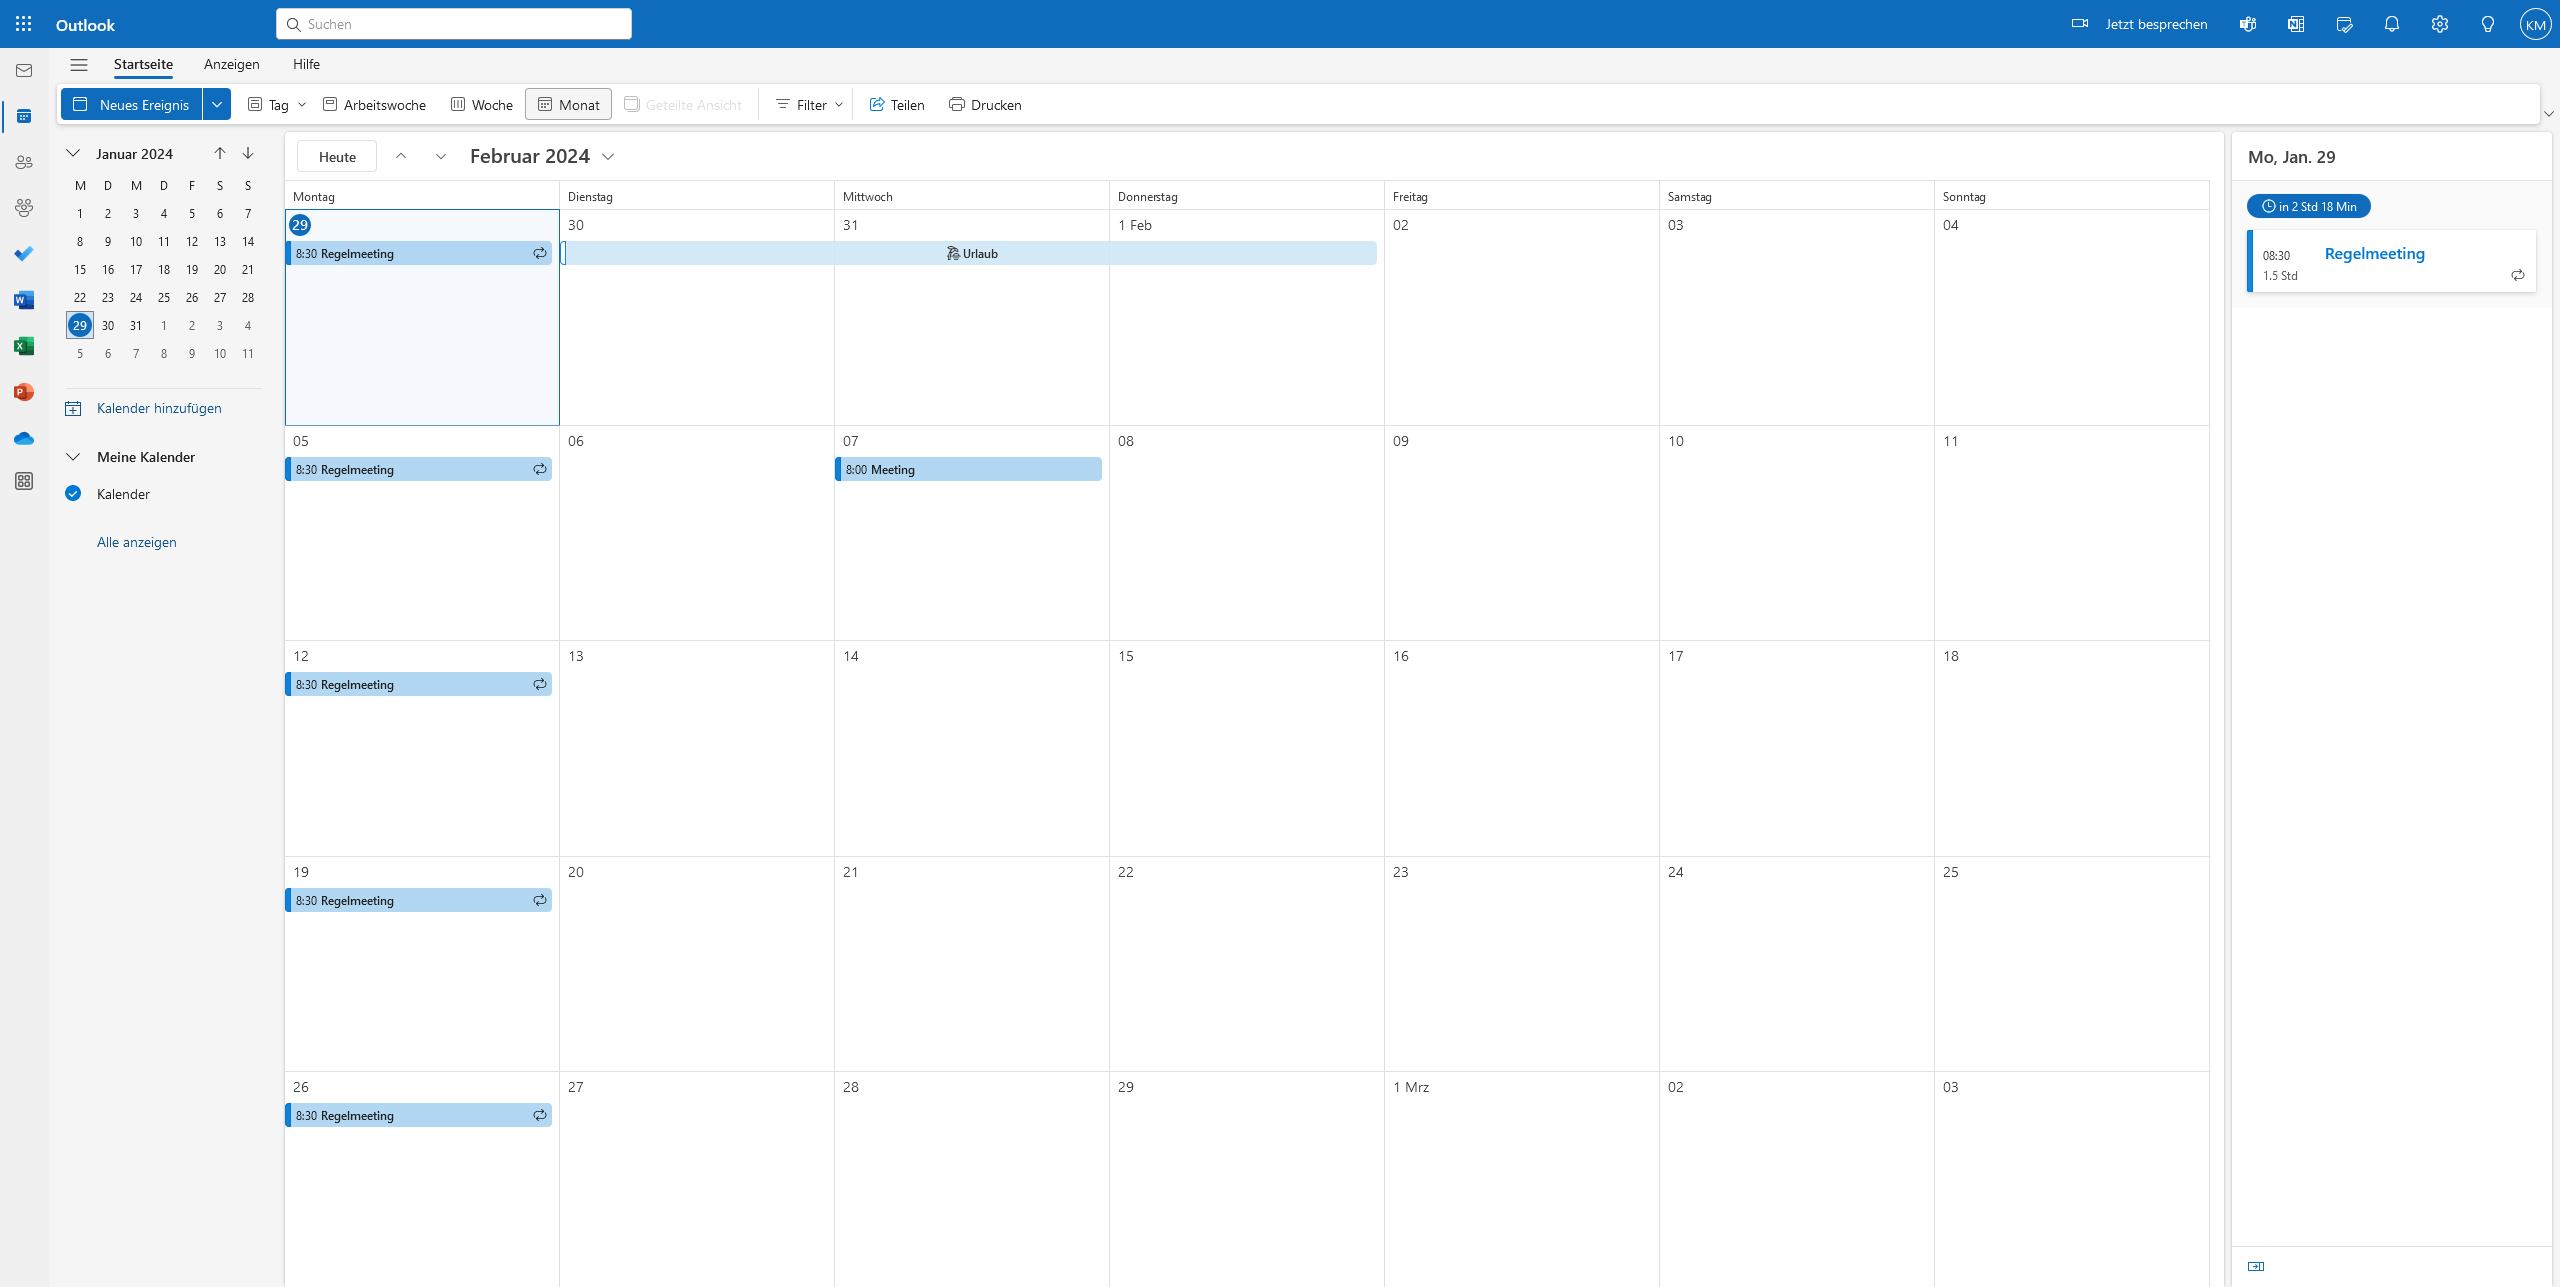
\includegraphics[width=0.75\textwidth]{images/OutlookLive_Calender1.png}
    \caption{Outlook-Live Kalender}
    \label{fig:outlook-live-calender}
\end{figure}

Eine weitere Hauptfunktion von Groupware-Systemen ist ein Kalender, der es Nutzern ermöglicht, Termine zu planen und Ereignisse in Form eines Kalenders zu organisieren (siehe Abbildung \ref{fig:outlook-live-calender}).
Die Terminplanung sollte es den Nutzern ermöglichen, andere Nutzer einzuladen, um die Zusammenarbeit und gemeinsame Organisation zu vereinfachen.
Auch das Anlegen von Regelterminen, das heißt Terminen, die regelmäßig wiederkehrend sind, sollte möglich sein.

\begin{figure}[H]
    \centering
    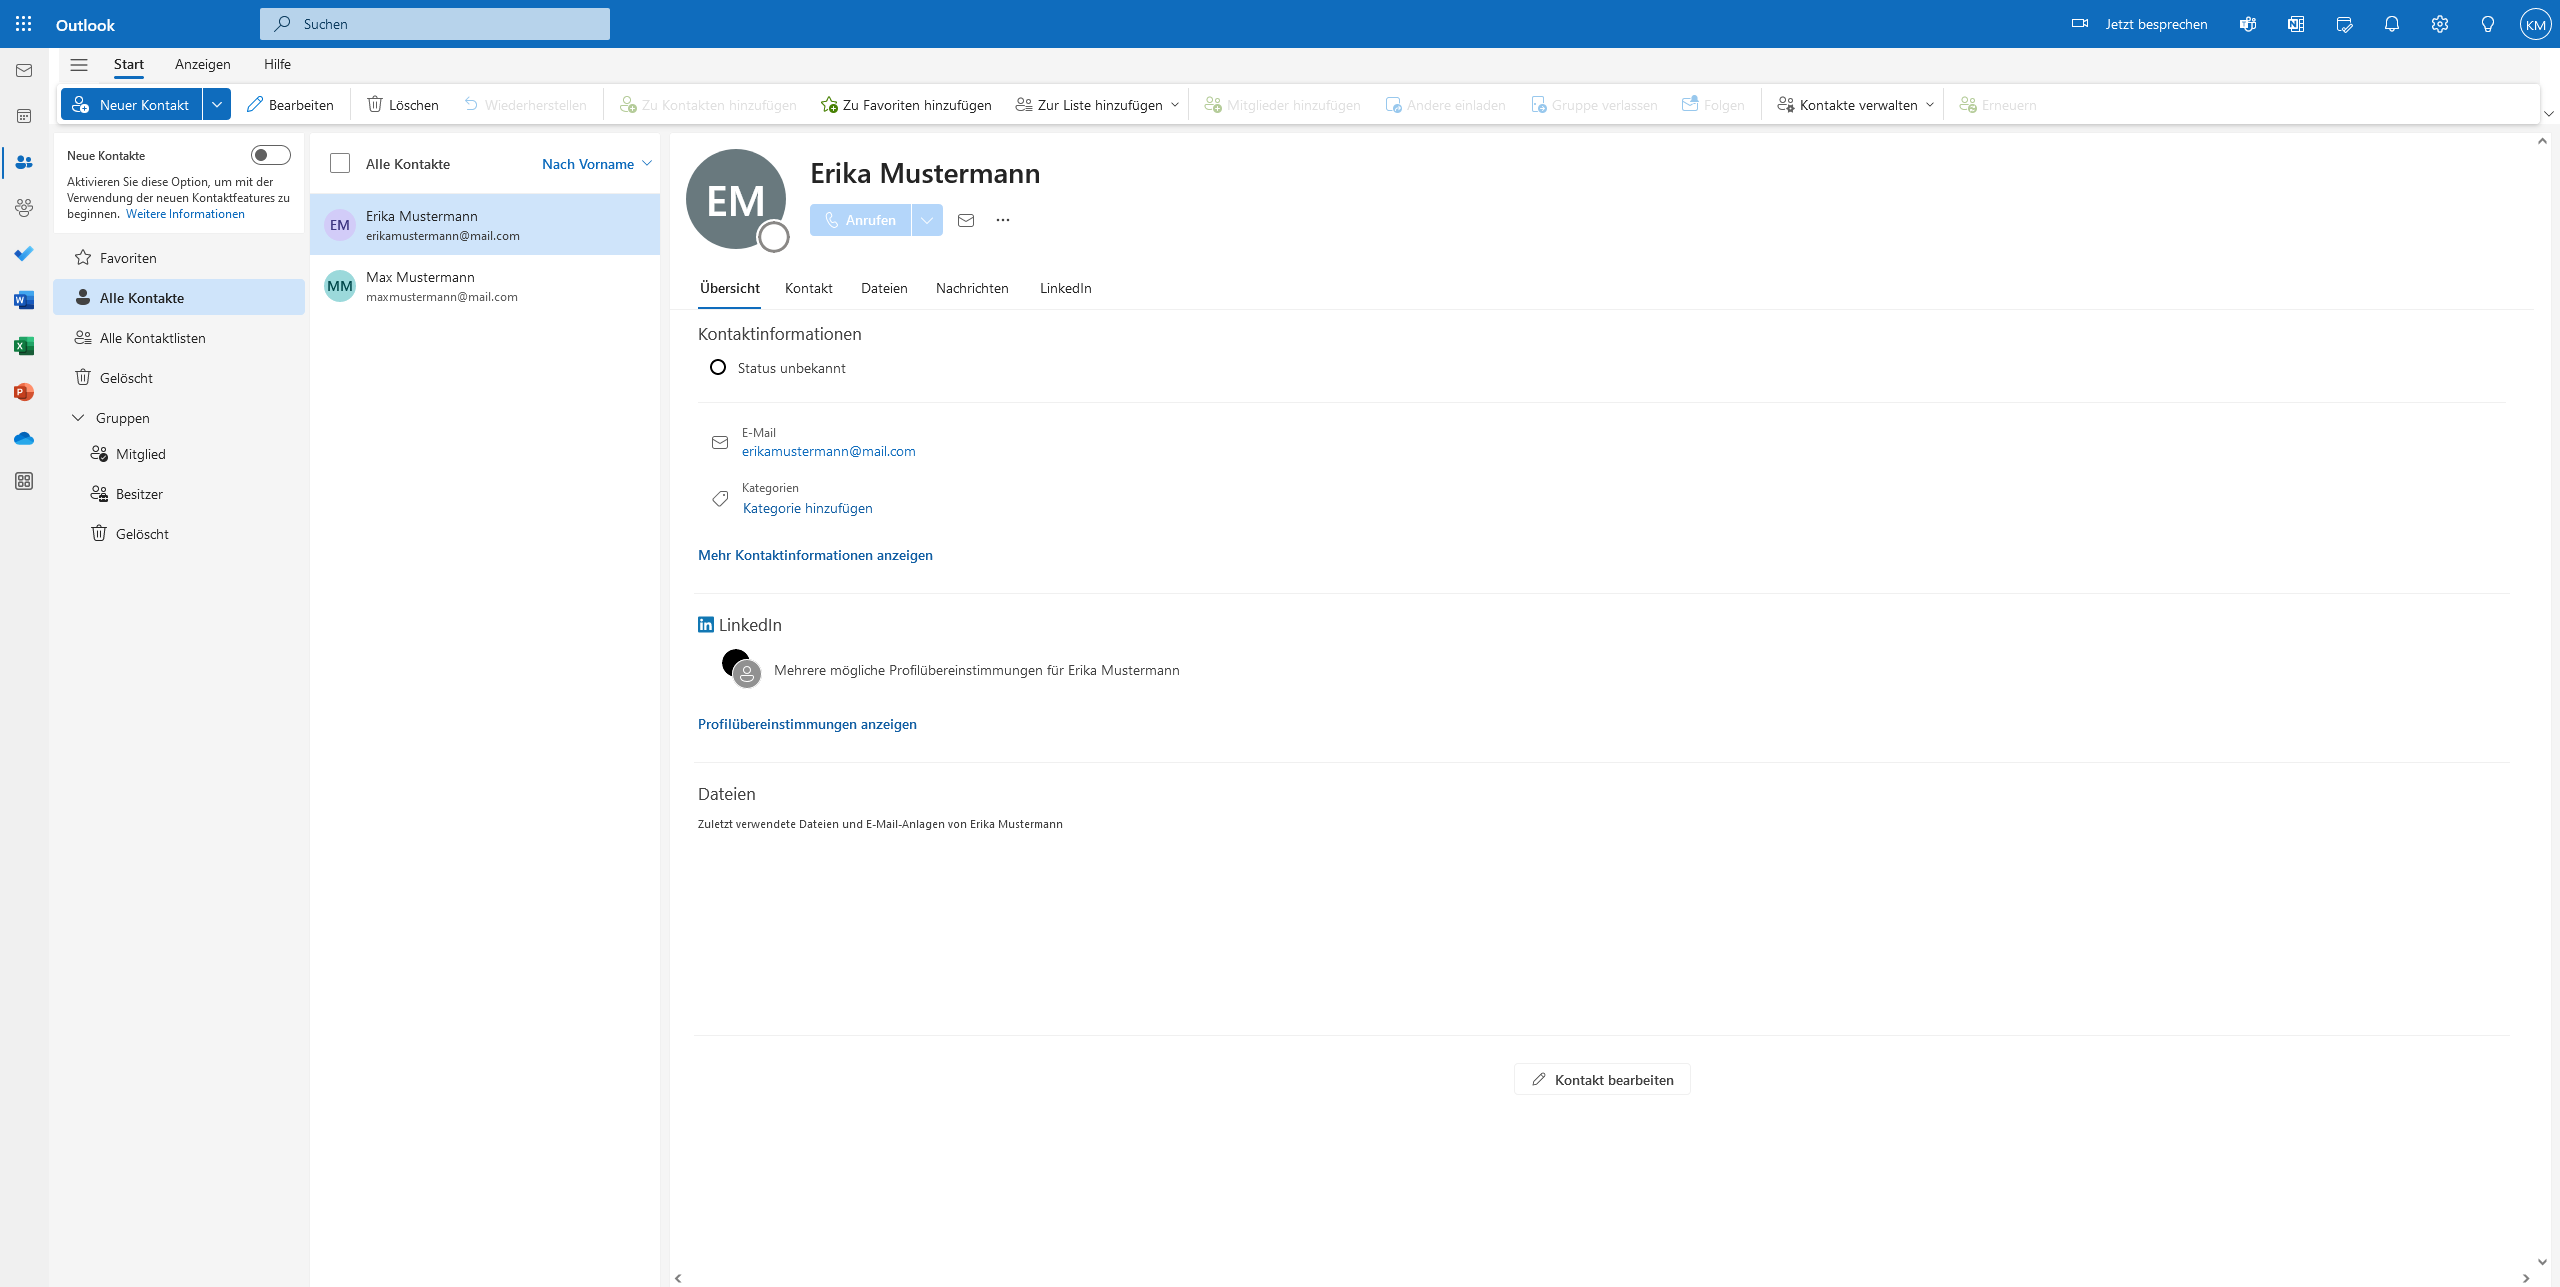
\includegraphics[width=0.75\textwidth]{images/OutlookLive_Contacts.png}
    \caption{Outlook-Live Kontakte}
    \label{fig:outlook-live-contacts}
\end{figure}

Kontakte sind ein weiterer wichtiger Bestandteil von Groupware-Systemen, um die Vernetzung innerhalb von Arbeitsgruppen zu organisieren.
Sie ermöglichen eine einfache Kontaktaufnahme zu anderen Gruppenmitgliedern.
In Outlook-Live kann man, wie in Abbildung \ref{fig:outlook-live-contacts} gezeigt, direkt vom Kontakt einer Person aus diese Person per Nachricht, Anruf oder E-Mail kontaktieren.


\section{Playwright}

Die Open-Source-Bibliothek Playwright, die Anfang 2020 von Microsoft veröffentlicht wurde, ermöglicht die gesteuerte Automatisierung von Browsern und Webinterfaces. Dadurch ist es möglich, Webanwendungen automatisiert zu testen oder Websites zu scannen.
Dabei bietet Playwright ein Application-Programming-Interface (API) für die Programmiersprachen JavaScript, TypeScript, Python, .NET und Java, sowie eine Vielzahl von Funktionen, die das Testen von Webanwendungen erleichtern.
Beispielsweise kann mit Playwright-Codegen die eigene Interaktion mit einer Webanwendung ausgezeichnet und als Code exportiert werden, der dann als Test für die ausgeführte Interaktion verwendet werden kann.
So können effizient Frontend-Tests für eine Vielzahl von Anwendungen implementiert werden.
\autocite[Quelle:][]{playwright}
\\
\\
Im Fall der Studienarbeit wurde Playwright verwendet, um automatisierte End-to-End-Tests für das final ausgewählte Groupware-System durchzuführen.
End-to-End-Tests können das korrekte Betriebsverhalten einer Anwendung sicherstellen, da sie Tests basierend auf dem Verhalten des Endnutzers sind.
Sie sind vor allem bei Anwendungen die viele Nutzerinteraktionen erfordern sinnvoll, da sie die Anwendung in einer realen Umgebung simulieren \autocite[vgl.][]{e2e-blog}.
Dabei werden Frontend-Tests implementiert, die typische Interaktionen mit der Benutzeroberfläche simulieren.
So können beispielsweise Formulare ausgefüllt oder Buttons angeklickt werden, womit ein Nutzer-Login und das anschließende Aufrufen der Mails des Nutzers simuliert werden kann.

Deckt man mit diesen Tests alle Funktionsbereiche des Groupware-Systems ab, kann man durch das Ausführen der Tests sicherstellen, dass die Anwendung nach einer Änderung noch wie erwartet funktioniert.
Auch falls die Anwendung in Zukunft unerwartete Ausfälle generiert, können diese durch flächendeckende Tests genauer erkannt werden, da sofort ersichtlich ist, welche Bereiche des Systems noch funktionieren und welche nicht.
Geht beispielsweise der zuvor erwähnte Test des aufrufen der Mails schief, gibt es mit hoher Wahrscheinlichkeit ein Problem mit der Verbindung zum Mail Server.
\\
Zudem können solche Tests in Playwright in verschiedenen Browsern (Chromium, Firefox, Safari) ausgeführt werden, wodurch die Funktionalität der Anwendung auch auf verschiedenen Browsern sichergestellt und kontinuierlich getestet werden kann.
Da die Groupware von einer Vielzahl von Systemen zugänglich sein soll, ist diese Funktion ein essenzieller Bestandteil der Testanforderungen.








